\scanpage{24}
% archive sheet number: 23
$A$ anneau local \inserted{\unsure{noeth|noeth.}} réduit de dim $2$,

de profondeur $\deleted{\unsure{=}}2$

$f\in\unsure{\mathfrak r|\mathfrak m}A$ tel que $A/fA$ est régulier

\noindent\begin{tikzpicture}[x=\linewidth,y=1em]
\draw (0,0) -- (.91,0); \draw (.82,1.6) -- (.82,-.8);
\end{tikzpicture}

\diagram{\begin{tikzcd}[ampersand replacement=\&,column sep=small,row sep=small]
\& X \arrow[dl] \arrow[d,dash] \& A\supset B\\
{} \& {} \& B\times B'
\end{tikzcd}}
\diagram{\begin{tikzcd}[ampersand replacement=\&,row sep=small]
B_{\eta} \& A_{\eta}\arrow[l,"\beta"'] \& B_{\eta}\arrow[l,"\alpha"']\arrow[ll,bend right=28,"N"']\\
B \& A\arrow[l]\arrow[u] \& B\arrow[l]
\end{tikzcd}}

$A_{\eta}=A_{1\eta}\times A_{2\eta}$ \quad $A$ OK.

\[
\begin{aligned}
B_1&=\overline{A_{1\eta}} \quad A \qquad X \qquad N_{\eta} \qquad A\unsure{\subset|\leftarrow}B\\
B_2&=\overline{A_{2\eta}}
\end{aligned}
\]

\diagram{\begin{tikzcd}[ampersand replacement=\&,row sep=small]
A \& \unsure{\text{---}|\rightarrow} \& \overline{A_{1\eta}}\\
A\arrow[rr] \& {} \& \overline{A_{2\eta}}
\end{tikzcd}}
\diagram{\begin{tikzcd}[ampersand replacement=\&,row sep=small]
\& A\arrow[r,shift right] \& \deleted{\unsure{A}}B_1\times B_2\arrow[l,shift right]\\
\deleted{B_1\times B_2}\arrow[ur] \& \&
\end{tikzcd}}

\diagram{\begin{tikzcd}[ampersand replacement=\&,row sep=small,column sep=small]
0\arrow[d] \& 0\arrow[d,dash] \& \overline A\\
A\arrow[u,shift left] \& \check A\arrow[d] \& {}\\
B\arrow[u] \& \unsure{\check B|\check D}\arrow[d] \& B\arrow[d]\\
C\arrow[u] \& \check C \& C
\end{tikzcd}}

\diagram{\begin{tikzcd}[ampersand replacement=\&,row sep=small]
\& T\arrow[dl]\\
A_{\unsure{.|\circ}}\&\deleted{B}\\
A_{\eta}\& B_{\eta}\arrow[l]\\
\&T_{\eta}\arrow[u]
\end{tikzcd}}

\figure{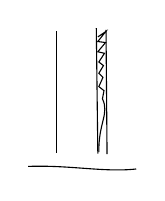
\begin{tikzpicture}[x=.65cm,y=.65cm]
\draw (0,.22)--(0,2.6);
\draw (.8,.2)--(.77,2.65) (.98,.19)--(.96,2.62);
\draw (.82,.23) .. controls (.81,.8) and (1.03,.98) .. (.89,1.27)
 --(.92,1.43)--(.82,1.51)--(.9,1.69)--(.82,1.77)--(.91,1.92)--(.82,1.99)
 --(.93,2.16)--(.8,2.19)--(.95,2.37)--(.8,2.39)--(.95,2.58)--(.8,2.48);
\draw (-.56,-.05) .. controls (.26,-.02) and (.93,-.17) .. (1.55,-.1);
\end{tikzpicture}}

\diagram{\begin{tikzcd}[ampersand replacement=\&,row sep=small]
A\arrow[d,very thick]\\ S
\end{tikzcd}}
